% +------------------------------------------------------------------------+
% | CGAL Reference Manual:  modifier.tex
% +------------------------------------------------------------------------+
% | Modifier Base Class for CGAL.
% |
% | 11.10.1996   Lutz Kettner
% |
% |
\RCSdef{\modifierRev}{$Revision$}
\RCSdefDate{\modifierDate}{$Date$}
% +------------------------------------------------------------------------+

\beforecprogskip\medskipamount
\aftercprogskip\medskipamount
\ccParDims

\chapter{Protected Access to Internal Representations}
\label{chapterModifier}
\ccChapterRelease{\modifierRev. \ \modifierDate}\\
\ccChapterAuthor{Lutz Kettner}

% +=========================================================================+
\section{Introduction}
% +=========================================================================+

High level data structures typically maintain integrity of an internal
data representation, which they protect from the user. A minimal while
complete interface of the data structure allows manipulations in the
domain of valid representations. Additional operations might benefit
from being allowed to access the internal data representation
directly. An example are intermediate steps within an algorithm where
the internal representation would be invalid. We present a general
method to accomplish access in a safe manner, such that the high level
data structures can guarantee validity after the possibly compromising
algorithm has finished its work. An example are polyhedral surfaces in
the Basic Library, where a construction process like for
a file scanner could be performed more efficiently on the internal
halfedge data structure than by using the high-level Euler operators
of the polyhedron.

\begin{figure}
\begin{ccTexOnly}
    \begin{center}
      \parbox{\textwidth}{%
          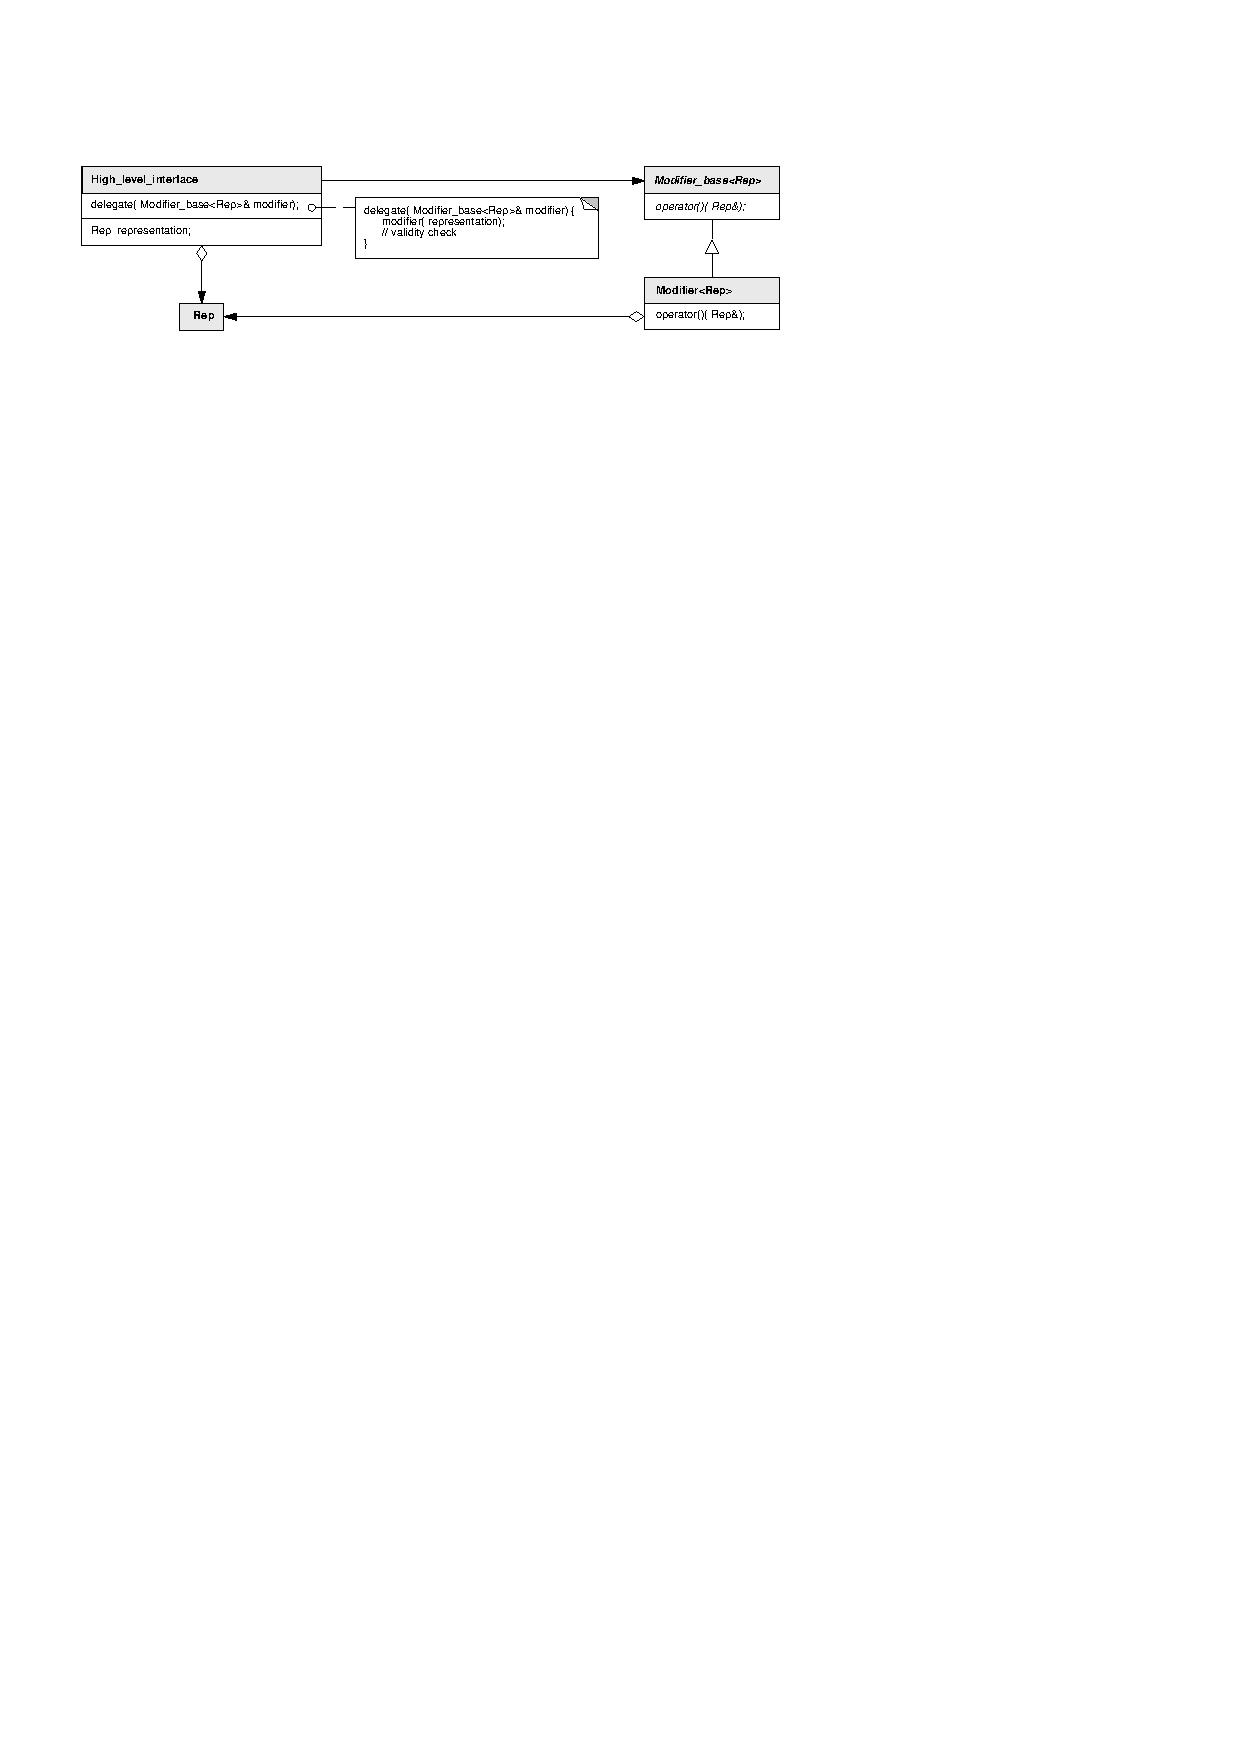
\includegraphics[width=\textwidth]{idraw/modifier.ips}%
      }
    \end{center}
\end{ccTexOnly}

    \caption{Class diagram for the modifier. It illustrates the
             safe access to an internal representation through an
             high-level interface.
    \label{figureModifierDesign}}

\begin{ccHtmlOnly}
    <CENTER>
    <A HREF="./modifier.gif">
        <img src="./modifier_small.gif" alt="Modifier Class Diagram"></A><BR>
    </CENTER>
\end{ccHtmlOnly}
\end{figure}

The solution provided here is inspired by the strategy
pattern~\cite{ghjv-dpero-95}, though it serves a different intent, see
Figure~\ref{figureModifierDesign}.  The abstract base class
\ccc{Modifier_base<R>} declares a pure virtual member function
\ccc{operator()} that accepts a single reference parameter of the
internal representation type. The member function \ccc{delegate()} of
the high-level interface calls this \ccc{operator()} with its internal
representation.  An actual modifier implements this virtual function,
thus gaining access to the internal representation. Once, the modifier
has finished its work, the member function \ccc{delegate()} is back in
control and can check the validity of the internal representation.
Summarizing, a user can implement and apply arbitrary functions based
on the internal representation and keeps the benefit if a protected
high-level interface. User provided modifiers must in any case return
a valid internal representation or the checker in the high-level
interface is allowed (and supposed) to abort the program. The
indirection via the virtual function invocation is negligible for
operations that consists of more than a pointer update or integer
addition.





% +--------------------------------------------------------+
\ccParDims
\beforecprogskip\parskip
\aftercprogskip0pt

% EOF


